% Options for packages loaded elsewhere
\PassOptionsToPackage{unicode}{hyperref}
\PassOptionsToPackage{hyphens}{url}
%
\documentclass[
  ignorenonframetext,
]{beamer}
\usepackage{pgfpages}
\setbeamertemplate{caption}[numbered]
\setbeamertemplate{caption label separator}{: }
\setbeamercolor{caption name}{fg=normal text.fg}
\beamertemplatenavigationsymbolsempty
% Prevent slide breaks in the middle of a paragraph
\widowpenalties 1 10000
\raggedbottom
\setbeamertemplate{part page}{
  \centering
  \begin{beamercolorbox}[sep=16pt,center]{part title}
    \usebeamerfont{part title}\insertpart\par
  \end{beamercolorbox}
}
\setbeamertemplate{section page}{
  \centering
  \begin{beamercolorbox}[sep=12pt,center]{part title}
    \usebeamerfont{section title}\insertsection\par
  \end{beamercolorbox}
}
\setbeamertemplate{subsection page}{
  \centering
  \begin{beamercolorbox}[sep=8pt,center]{part title}
    \usebeamerfont{subsection title}\insertsubsection\par
  \end{beamercolorbox}
}
\AtBeginPart{
  \frame{\partpage}
}
\AtBeginSection{
  \ifbibliography
  \else
    \frame{\sectionpage}
  \fi
}
\AtBeginSubsection{
  \frame{\subsectionpage}
}
\usepackage{amsmath,amssymb}
\usepackage{lmodern}
\usepackage{iftex}
\ifPDFTeX
  \usepackage[T1]{fontenc}
  \usepackage[utf8]{inputenc}
  \usepackage{textcomp} % provide euro and other symbols
\else % if luatex or xetex
  \usepackage{unicode-math}
  \defaultfontfeatures{Scale=MatchLowercase}
  \defaultfontfeatures[\rmfamily]{Ligatures=TeX,Scale=1}
\fi
\usetheme[]{Frankfurt}
\usecolortheme{beaver}
% Use upquote if available, for straight quotes in verbatim environments
\IfFileExists{upquote.sty}{\usepackage{upquote}}{}
\IfFileExists{microtype.sty}{% use microtype if available
  \usepackage[]{microtype}
  \UseMicrotypeSet[protrusion]{basicmath} % disable protrusion for tt fonts
}{}
\makeatletter
\@ifundefined{KOMAClassName}{% if non-KOMA class
  \IfFileExists{parskip.sty}{%
    \usepackage{parskip}
  }{% else
    \setlength{\parindent}{0pt}
    \setlength{\parskip}{6pt plus 2pt minus 1pt}}
}{% if KOMA class
  \KOMAoptions{parskip=half}}
\makeatother
\usepackage{xcolor}
\IfFileExists{xurl.sty}{\usepackage{xurl}}{} % add URL line breaks if available
\IfFileExists{bookmark.sty}{\usepackage{bookmark}}{\usepackage{hyperref}}
\hypersetup{
  pdftitle={Models for autocorrelated data},
  pdfauthor={Vojtěch Barták},
  hidelinks,
  pdfcreator={LaTeX via pandoc}}
\urlstyle{same} % disable monospaced font for URLs
\newif\ifbibliography
\usepackage{graphicx}
\makeatletter
\def\maxwidth{\ifdim\Gin@nat@width>\linewidth\linewidth\else\Gin@nat@width\fi}
\def\maxheight{\ifdim\Gin@nat@height>\textheight\textheight\else\Gin@nat@height\fi}
\makeatother
% Scale images if necessary, so that they will not overflow the page
% margins by default, and it is still possible to overwrite the defaults
% using explicit options in \includegraphics[width, height, ...]{}
\setkeys{Gin}{width=\maxwidth,height=\maxheight,keepaspectratio}
% Set default figure placement to htbp
\makeatletter
\def\fps@figure{htbp}
\makeatother
\setlength{\emergencystretch}{3em} % prevent overfull lines
\providecommand{\tightlist}{%
  \setlength{\itemsep}{0pt}\setlength{\parskip}{0pt}}
\setcounter{secnumdepth}{-\maxdimen} % remove section numbering
\AtBeginSubsection{}
\ifLuaTeX
  \usepackage{selnolig}  % disable illegal ligatures
\fi

\title{Models for autocorrelated data}
\author{Vojtěch Barták}
\date{LS 2022}

\begin{document}
\frame{\titlepage}

\begin{frame}[allowframebreaks]
  \tableofcontents[hideallsubsections]
\end{frame}
\hypertarget{general-overview}{%
\section{General overview}\label{general-overview}}

\hypertarget{general-model-for-spatial-data}{%
\subsection{General model for spatial
data}\label{general-model-for-spatial-data}}

\begin{frame}{General model for spatial data}
\small

\[\boldsymbol{Y}(\boldsymbol{s})=\boldsymbol{\mu}(\boldsymbol{s})+\boldsymbol{e}(\boldsymbol{s})\]

\(\boldsymbol{Y}\) \ldots{} vector of response observations\\
\(\boldsymbol{s}\) \ldots{} vector of spatial coordinates\\
\(\boldsymbol{\mu}\) \ldots{} deterministic mean function\\
\(\boldsymbol{e}\) \ldots{} random ``error'' component

The spatial structure observed in \(\boldsymbol{Y}\) can be modelled:

\begin{itemize}
\tightlist
\item
  in the \textbf{mean component}

  \begin{itemize}
  \tightlist
  \item
    Spatially structured predictors (induced spatial structure)
  \item
    Autocovariate models
  \item
    Trend surface models
  \item
    Moran's eigenvector mapping
  \end{itemize}
\item
  in the \textbf{random component}

  \begin{itemize}
  \tightlist
  \item
    Geostatistical models
  \item
    Autoregressive models
  \end{itemize}
\item
  both
\end{itemize}
\end{frame}

\hypertarget{modeling-spatial-structure-in-the-mean-component}{%
\subsection{Modeling spatial structure in the mean
component}\label{modeling-spatial-structure-in-the-mean-component}}

\begin{frame}{Modeling spatial structure in the mean component}
\small

Linear models:

\begin{center}
$\boldsymbol{\mu}(\boldsymbol{s}) = \boldsymbol{X}(\boldsymbol{s})\boldsymbol{\beta}$,   $\boldsymbol{e}(\boldsymbol{s}) \sim MVN(\boldsymbol{0},\sigma^2\boldsymbol{I})$
\end{center}

\(\boldsymbol{X}(\boldsymbol{s})\) \ldots{} matrix of fixed predictors,
including spatially structured ones\\
\(\boldsymbol{\beta}\) \ldots{} vector of unknown parameters (fixed
effects)

\begin{itemize}
\tightlist
\item
  estimation by \emph{ordinary least squares} (OLS)
\end{itemize}

Generalized linear models:

\begin{enumerate}
\tightlist
\item
  \(Y_i\) are mutually independent, following a common distributional
  family (Gaussian, Poisson, Binomial, \ldots)
\item
  \(\boldsymbol{\mu(\boldsymbol{s})} = u[\boldsymbol{X}(\boldsymbol{s})\boldsymbol{\beta}]\),
  \(u\) \ldots{} link function
\end{enumerate}

\begin{itemize}
\tightlist
\item
  estimation by maximum likelihood (ML)
\end{itemize}
\end{frame}

\hypertarget{modeling-spatial-structure-in-the-random-component}{%
\subsection{Modeling spatial structure in the random
component}\label{modeling-spatial-structure-in-the-random-component}}

\begin{frame}{Modeling spatial structure in the random component}
\small

\[\boldsymbol{e} \sim (\boldsymbol{0}, \boldsymbol{\Sigma}(\boldsymbol{\theta}))\]

\begin{itemize}
\tightlist
\item
  \(\boldsymbol{\Sigma}\) is a positive definite matrix with at least
  some non-zero off-diagonal elements
\item
  \(\boldsymbol{\theta}\) is a vector o parameters describing the
  spatial dependence
\item
  Trying to capture the nature of spatial dependence - the real spatial
  autocorrelation
\item
  Relies on \textbf{stationarity} assumption
\item
  Fixed effects can be estimated by \emph{generalized least squares}
  (GLS)
\item
  Can be viewed as \textbf{mixed models} (estimation by ML/REML)
\end{itemize}
\end{frame}

\hypertarget{models-with-correlated-errors}{%
\section{Models with correlated
errors}\label{models-with-correlated-errors}}

\hypertarget{geostatistical-linear-model}{%
\subsection{Geostatistical linear
model}\label{geostatistical-linear-model}}

\begin{frame}{Geostatistical linear model}
\small

\[\boldsymbol{\mu}(\boldsymbol{s}) = \boldsymbol{X}(\boldsymbol{s})\boldsymbol{\beta}\]
\[\boldsymbol{e}(\boldsymbol{s}) = \boldsymbol{S}(\boldsymbol{s})+\boldsymbol{\epsilon}(\boldsymbol{s})\]

\(\boldsymbol{S}(\boldsymbol{s})\sim MVN(\boldsymbol{0}, \boldsymbol{C})\)
\ldots{} Gaussian process\\
\(\boldsymbol{C} = (\sigma_{i,j})\),
\(\sigma_{i,j} = Cov(S_i, S_j) = C(u)\) \ldots{} Covariance function\\
\(\boldsymbol{\epsilon}(\boldsymbol{s}) \sim MVN(\boldsymbol{0}, \tau^2\boldsymbol{I})\)
\ldots{} Nugget effect\\
\(\boldsymbol{\Sigma} = \boldsymbol{C}+\tau^2\boldsymbol{I}\)

Covariance function estimated from data:

\begin{itemize}
\tightlist
\item
  by fitting the curve to the sample variogram (\emph{classical
  geostatistics})
\item
  by ML/REML techniques together with other parameters
  (\emph{model-based approach})
\end{itemize}
\end{frame}

\hypertarget{geostatistical-linear-model-1}{%
\subsection{Geostatistical linear
model}\label{geostatistical-linear-model-1}}

\begin{frame}{Geostatistical linear model}
\small

Spatial prediction/interpolation: \textbf{kriging}
\[\hat{Y}(\boldsymbol{s}_0) = \boldsymbol{x}'\hat{\boldsymbol{\beta}}_{GLS}+\boldsymbol{c}'\boldsymbol{\Sigma}^{-1}(\boldsymbol{Y}-\boldsymbol{X}\hat{\boldsymbol{\beta}}_{GLS})\]

\(\boldsymbol{c} = (C(\boldsymbol{s}_0, \boldsymbol{s}_1),C(\boldsymbol{s}_0, \boldsymbol{s}_2),...,C(\boldsymbol{s}_0, \boldsymbol{s}_n))'\)\\
\(\boldsymbol{c}'\boldsymbol{\Sigma}^{-1}\) \ldots{} \emph{kriging
weights}\\
\(var(\hat{Y}(\boldsymbol{s}_0))\) \ldots{} \emph{kriging variance}

\begin{itemize}
\tightlist
\item
  Simple kriging \ldots{} known constant mean
\item
  Ordinary kriging \ldots{} unknown constant mean
\item
  Universal kriging \ldots{} unknown mean depending on covariates
\end{itemize}
\end{frame}

\hypertarget{geostatistical-glm}{%
\subsection{Geostatistical GLM}\label{geostatistical-glm}}

\begin{frame}{Geostatistical GLM}
\small

Generalized linear model (GLM):

\begin{enumerate}
\tightlist
\item
  \(Y_i\) \ldots{} mutually independent Gaussian/Poisson/Binomial
  variables
\item
  \(\boldsymbol{\mu(\boldsymbol{s})} = u[\boldsymbol{X}(\boldsymbol{s})\boldsymbol{\beta}]\),
  \(u\) \ldots{} link function
\end{enumerate}

Generalized linear geostatistical model (GLGM):

\begin{enumerate}
\tightlist
\item
  \(Y_i\) \ldots{} mutually independent Gaussian/Poisson/Binomial
  variables
\item
  \(\boldsymbol{\mu(\boldsymbol{s})} = u[\boldsymbol{X}(\boldsymbol{s})\boldsymbol{\beta} + \boldsymbol{S}(\boldsymbol{s})]\),
  \(u\) \ldots{} link function
\item
  \(\boldsymbol{S}(\boldsymbol{s})\) \ldots{} Gaussian process with zero
  mean and some covariance function
\end{enumerate}

\begin{itemize}
\tightlist
\item
  Special case of GLMM
\end{itemize}
\end{frame}

\hypertarget{autoregressive-models}{%
\subsection{Autoregressive models}\label{autoregressive-models}}

\begin{frame}{Autoregressive models}
\small

\begin{itemize}
\tightlist
\item
  Based on discrete locations with a \textbf{neighborhood structure}
\item
  Magnitude of spatial interactions between neighbors -\textgreater{}
  \textbf{spatial weights}
\end{itemize}

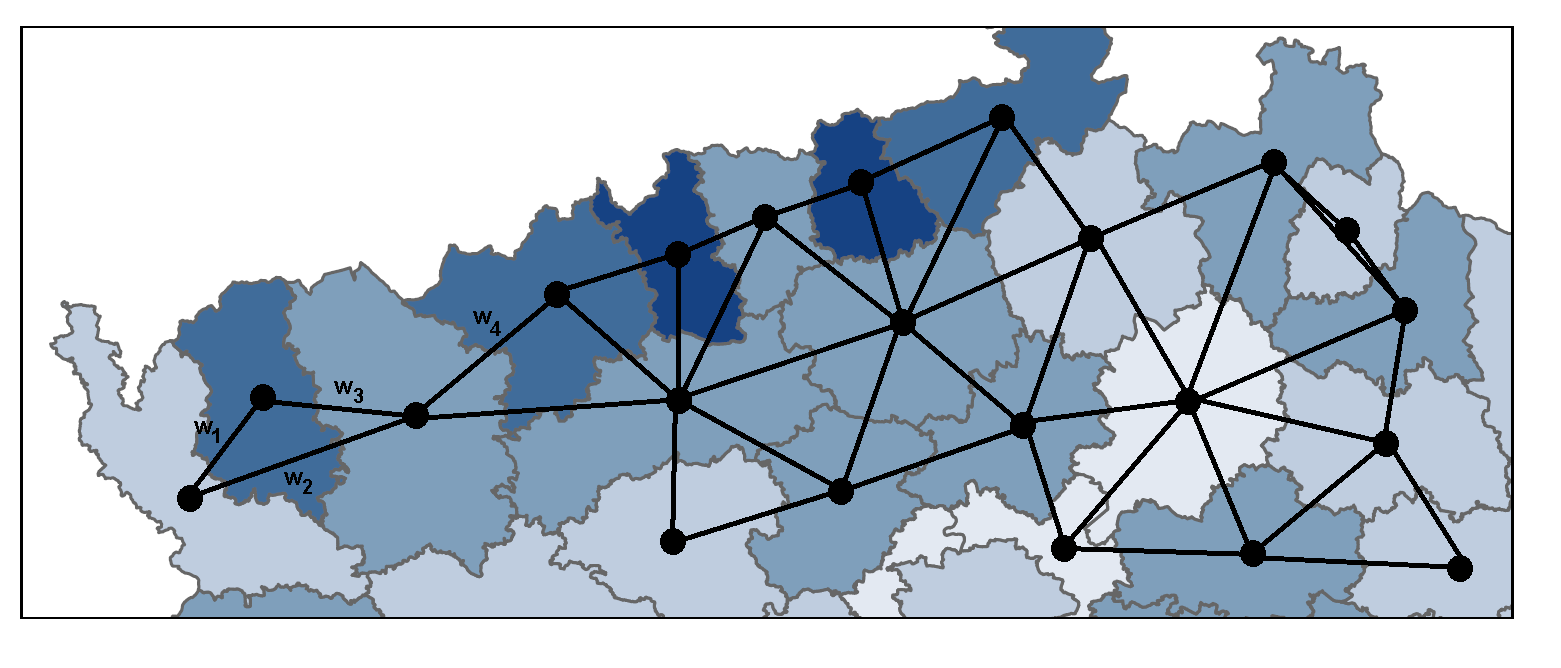
\includegraphics{areal_data.png}

\begin{itemize}
\tightlist
\item
  Not necessarily areal data\ldots{}
\end{itemize}
\end{frame}

\hypertarget{simultanuous-autoregressive-model}{%
\subsection{Simultanuous autoregressive
model}\label{simultanuous-autoregressive-model}}

\begin{frame}{Simultanuous autoregressive model}
\small

\[\boldsymbol{Y}(\boldsymbol{s}) = \boldsymbol{X}(\boldsymbol{s})\boldsymbol{\beta} + \boldsymbol{e}(\boldsymbol{s})\]
\[\boldsymbol{e}(\boldsymbol{s}) = \boldsymbol{B}\boldsymbol{e}(\boldsymbol{s})+\boldsymbol{\epsilon}(\boldsymbol{s})\]

\(\boldsymbol{B}\) \ldots{} matrix of spatial dependence parameters,
\(b_{i,i}=0\)\\
\(\boldsymbol{\epsilon}(\boldsymbol{s})\sim N(\boldsymbol{0}, \sigma^2\boldsymbol{I})\)\\
\(\boldsymbol{\Sigma}_{SAR}=(\boldsymbol{I}-\boldsymbol{B})^{-1}\sigma^2\boldsymbol{I}(\boldsymbol{I}-\boldsymbol{B}')^{-1}\)

Usually:

\[\boldsymbol{B} = \rho\boldsymbol{W}\]

\(\rho\) \ldots{} single correlation parameter\\
\(\boldsymbol{W}\) \ldots{} matrix of spatial weights
\end{frame}

\hypertarget{conditional-autoregressive-model}{%
\subsection{Conditional autoregressive
model}\label{conditional-autoregressive-model}}

\begin{frame}{Conditional autoregressive model}
\small

Assumption: Spatial process is \emph{Markov random field}

\[E[Y(\boldsymbol{s}_i)|\boldsymbol{Y}(\boldsymbol{s})_{-i}]=\boldsymbol{x}(\boldsymbol{s}_i)'\boldsymbol{\beta} + \sum_{j=1}^nb_{i,j}[Y(\boldsymbol{s}_j) - \boldsymbol{x}(\boldsymbol{s}_j)'\boldsymbol{\beta}]\]
\[Var[Y(\boldsymbol{s}_i)|\boldsymbol{Y}(\boldsymbol{s})_{-i}] = \sigma^2\]

\begin{itemize}
\tightlist
\item
  \(\boldsymbol{\Sigma}_{CAR}=(\boldsymbol{I}-\boldsymbol{B})^{-1}\sigma^2\)
\item
  Again, usually \(\boldsymbol{B} = \rho\boldsymbol{W}\)
\item
  In these constant-variance versions, every SAR model can be expressed
  as a CAR model, and vice versa
\end{itemize}
\end{frame}

\hypertarget{models-with-uncorrelated-errors}{%
\section{Models with uncorrelated
errors}\label{models-with-uncorrelated-errors}}

\hypertarget{autocovariate-models}{%
\subsection{Autocovariate models}\label{autocovariate-models}}

\begin{frame}{Autocovariate models}
\small

\begin{itemize}
\item
  Each observation is modeled as depending on a summary of neighboring
  observations
\item
  This \emph{autocovariate} is prepared first a added as a fixed
  predictor
\item
  A ``naive'' approach to autoregression
\item
  Typically a weighted average of the neighboring values
\item
  Can be used in any type of model (G)L(M)M, GAM, Random Forests,
  \ldots)
\item
  Assumes stationarity
\end{itemize}
\end{frame}

\hypertarget{trend-surface-models}{%
\subsection{Trend surface models}\label{trend-surface-models}}

\begin{frame}[fragile]{Trend surface models}
\small

\begin{itemize}
\item
  Originally: a simple (linear, quadratic) spatial trend is added as
  fixed predictor
\item
  Combined with geostatistical models
\item
  Extended to complex, nonlinear smooth surfaces, describing the
  unexplained spatial structure
\item
  Typically a smooth term \texttt{s(x,\ y)} in a \textbf{generalized
  additive model} (GAM)
\end{itemize}

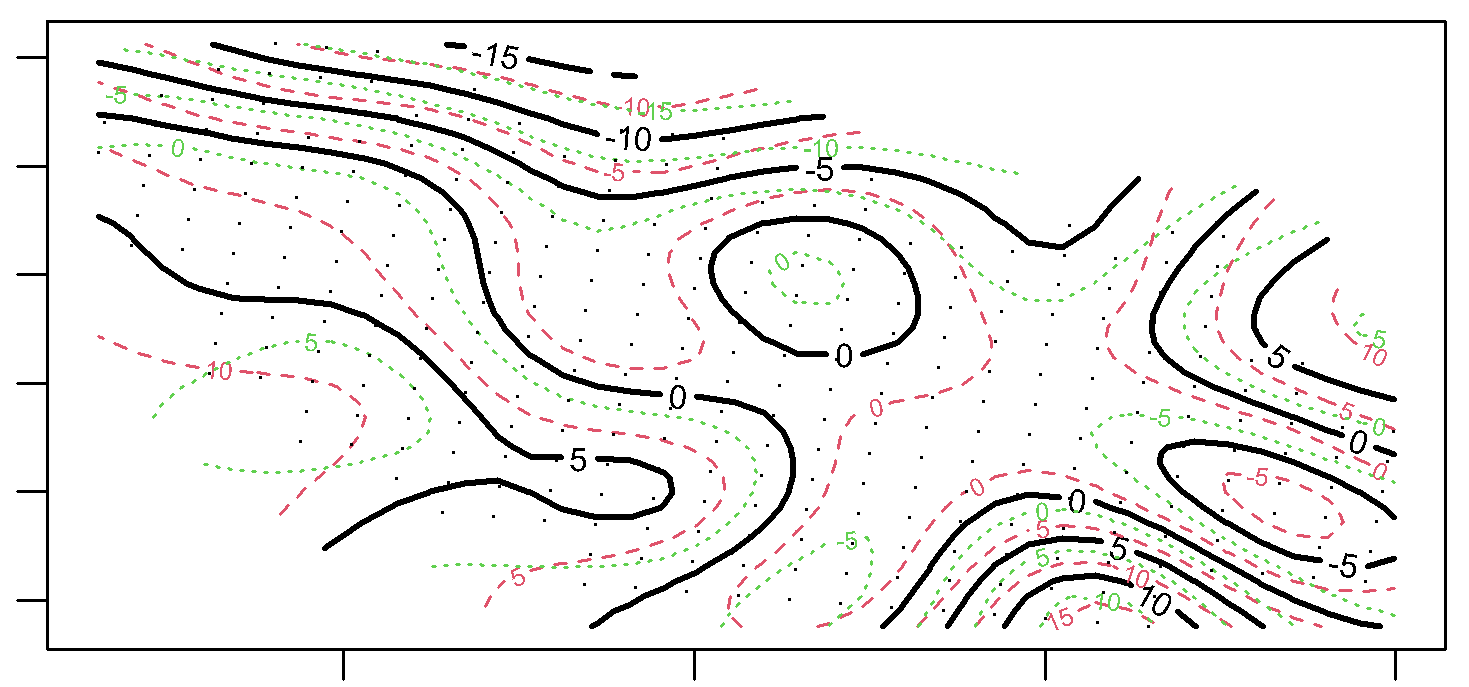
\includegraphics[width=0.4\textwidth,height=\textheight]{spline_surf.png}

\begin{itemize}
\tightlist
\item
  Description, but not explanation!
\item
  \textbf{Does not assume stationarity!}
\end{itemize}
\end{frame}

\hypertarget{morans-eigenvectors-mapping}{%
\subsection{Moran's eigenvectors
mapping}\label{morans-eigenvectors-mapping}}

\begin{frame}{Moran's eigenvectors mapping}
\small

\begin{itemize}
\tightlist
\item
  PCA applied to the distance or weight matrix
\item
  The resulting variables (called Moran's eigenvectors) used as fixed
  predictors
\item
  Only those associated with positive eigenvalues (positive spatial
  dependence)
\end{itemize}

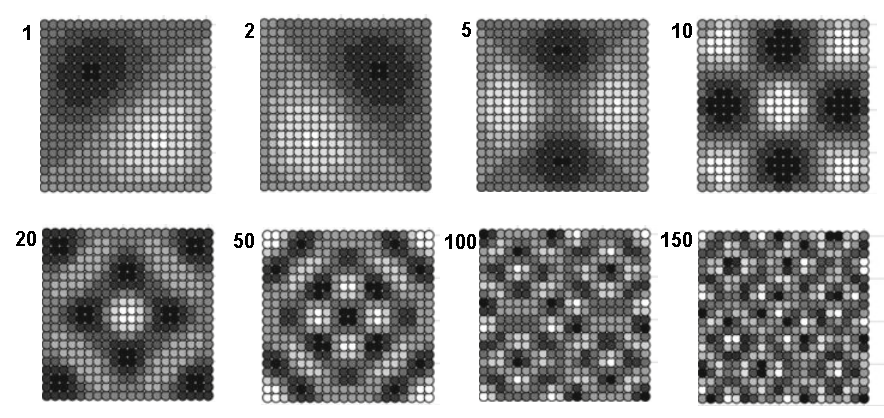
\includegraphics[width=0.7\textwidth,height=\textheight]{moran_eigs.png}

\begin{itemize}
\tightlist
\item
  Similar to trend surface models and Fourier transform
\item
  Significant eigenvectors represent spatial dependence at different
  scales
\end{itemize}
\end{frame}

\end{document}
